\qns{Filter Design}
\qcontributor{Maxwell Chen}

Suppose you have been hired to design a biomedical sensor that can detect and output recordings of Alpha brainwaves in the frequency range $8 \, \text{Hz}$ to $13 \, \text{Hz}$. 
Unfortunately, our sensor is faulty: it is also picking up Gamma brainwaves in the frequency range $32 \, \text{Hz}$ to $100 \, \text{Hz}$, interfering with our ability to get clean recordings of alpha brainwaves. 
We want to create a new design for our sensor that can remove this interference, giving us a clearer signal.

\begin{enumerate}

	\qitem What kind of filter could you use to remove this interference? 
    
    \sol { 
    We should use a low-pass filter. The interference is at a higher frequency than our desired signal, so we filter out the higher frequencies and keep the lower frequencies.
    }
	
	\qitem Assume we only have access to resistors and capacitors. \textbf{Sketch the corresponding filter circuit and write out its transfer function.} 

	\sol {
	$$H(\omega) = \frac{\widetilde{Z_{out}}}{\widetilde{Z_{in}}} = \frac{\frac{1}{j\omega C}}{R + \frac{1}{j \omega C}} = \frac{1}{1 + j\omega RC} = \frac{1}{1 + j \frac{\omega}{\omega_p}}$$.

	\begin{center}
  \begin{circuitikz} \draw
    (0, 0) node[ground] {}
      to [sV, l_=$V_{in}$] (0, 4)
      to [R = R] (4, 4)
      to [C = C] (4, 0)
      node[ground] {}

    (4, 3) to[short, -o] (6, 3) node[anchor=west] (A) {A}

    (4, 1) to[short, -o] (6, 1) node[anchor=west] (B) {B}

    (A) to[open, l^=$V_{out}$] (B)
  ;\end{circuitikz}
\end{center}

	}	

	\qitem $\omega_p = \frac{1}{RC}$ is the pole frequency which determines the frequency at which our filter starts attenuating the signal. \textbf{Should we maximize or minimize $\omega_p$ to remove as much of the interference as possible?}

	\sol {
	We should minimize the pole frequency. The transfer function will start filtering frequencies sooner, meaning that we maximize the amount by which higher frequencies are attenuated.
	}	

	\qitem Say we can set our cutoff frequency to $10 \, \text{Hz}$, $20 \, \text{Hz}$, $32 \, \text{Hz}$, $100 \, \text{Hz}$, or $120 \, \text{Hz}$. Which is the best pole frequency, and why?

	\sol {
	20Hz. This is the lowest pole frequency we can choose; the Gamma brainwaves will be attenuated more if we choose 20Hz than 32Hz because the transfer function will start filtering at a lower frequency. 10Hz is too low and risks cutting off Alpha brainwaves.
	}	

	\qitem We only have a 3.3 k$\Omega$ resistor in our workstation. What capacitor value should we use for our filter?

	\sol {
	If we want a pole frquency of 20Hz, then $f = \frac{\omega_p}{2 \pi} = \frac{1}{2 \pi RC} = 20Hz$. So, $C = \frac{1}{2 \pi \cdot 33 \cdot 10^{3} \Omega \cdot 20Hz} = 2.41 \, \mu$F.
	}	

	\qitem Draw the Bode plot for the magnitude and phase response of this filter.

	\sol {
		\begin{figure}[h]
		\centering
		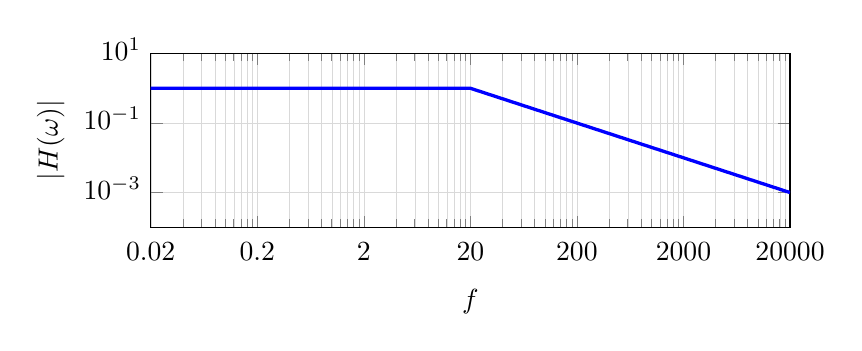
\begin{tikzpicture}[
		  declare function={
			mag(\omega)= (\omega < 10^8) * (1) +
					  (\omega >= 10^8) * (10^8 / \omega)
		   ;
		  }
		]
		  \begin{loglogaxis}[
		  	typeset ticklabels with strut,
			ymin=0.0001, ymax=10, ylabel=$|H(\omega)|$,
			xmin=10^5, xmax=10^11, xlabel=$f$,
			xticklabels={$0.02$,$0.2$,$2$,$20$,$200$, $2000$, $20000$},
			domain=10^5:10^11,
			grid=both, grid style={line width=.1pt, draw=gray!30},
			width=\textwidth * 0.8,
			height=\textwidth / 3.2
		  ]
			\addplot [blue,very thick] {mag(x)};
		  \end{loglogaxis}
		\end{tikzpicture}
		\end{figure}

		\begin{figure}[h]
		\centering
		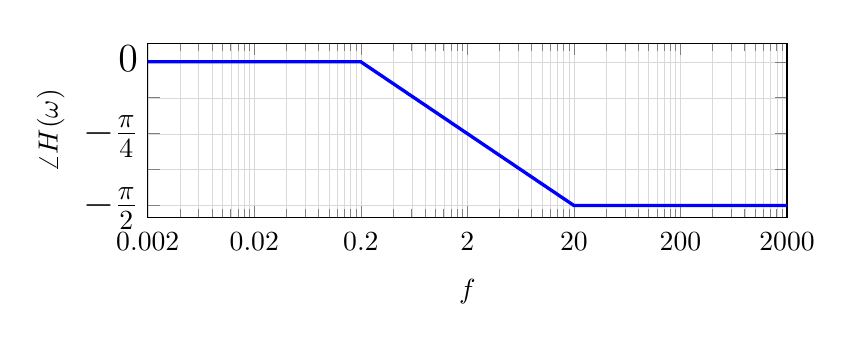
\begin{tikzpicture}[
		  declare function={
			phase(\omega)= (\omega < 10^7) * (0) +
					  and(\omega >= 10^7, \omega < 10^9) * (-pi / 4 * (log10(\omega) - 7)) +
					  (\omega >= 10^9) * (-pi / 2)
		   ;
		  }
		]
		  \begin{semilogxaxis}[
		  	typeset ticklabels with strut,
			ymin= -1.7, ymax=0.2, ylabel=$\angle H(\omega)$,
			ytick={-pi/2, -3*pi/8, -pi/4, -pi/8, 0},
			yticklabel style={font=\Large},
			yticklabels={$-\frac{\pi}{2}$, $\,$, $-\frac{\pi}{4}$, $\,$, $0$},
			xticklabels={$0.002$,$0.02$,$0.2$,$2$,$20$, $200$, $2000$},
			xmin=10^5, xmax=10^11, xlabel=$f$,
			domain=10^5:10^11,
			grid=both, grid style={line width=.1pt, draw=gray!30},
			width=\textwidth * 0.8,
			height=\textwidth / 3.2
		  ]
			\addplot [blue,very thick] {phase(x)};
		  \end{semilogxaxis}
		\end{tikzpicture}
		\end{figure}
	}	

	\qitem \textbf{(Optional:)} Say that our filter is successful at removing the interference we initially detected. We now notice that there is another source of interference--Delta brainwaves--in the frequency range 0.5Hz to 4Hz. \textbf{How could we modify our design to remove both sources of interference and get a clear recording of Alpha brainwaves?}

	\sol {
	Replace our low-pass filter with a bandpass filter. This will attenuate both sources of noise and leave our frequency band for Alpha brainwaves intact for our sensor to record.
	}	

\end{enumerate}